\problemname{Snow Wall Inspector}
The PO jury cannot program. After the fiasco in the online qualification, where the broken judge for the problem \href{https://pokval16.kattis.com/problems/pokval16.snomur}{Snow Wall} accidentally gave Iceland the win with 211.58 out of 100 points on the problem, the jury has decided to outsource its judges to people who can actually code --- PO finalists.

The problem was as follows:

Sweden is building a snow wall of a certain width $W$.
As building material, there are a number of snow blocks that all have height 1, but can have different widths.
When the wall is constructed, each block must satisfy the following rule: on the row below the block,
at the two positions where the block has its endpoints, there must be a block immediately to the right and left of the point,
except at the beginning and end of a row, where there must instead be an endpoint \emph{on every row} (see the left, second-from-top wall in Figure~\ref{fig:sample} where this is missing on the top row).

Furthermore, there must not be a gap at the same position on two directly consecutive rows \emph{in the wall} (the empty row
just above the wall does not count).

The following image illustrates some invalid (left) and valid (right) walls:

\begin{figure}[h]
	\centering
	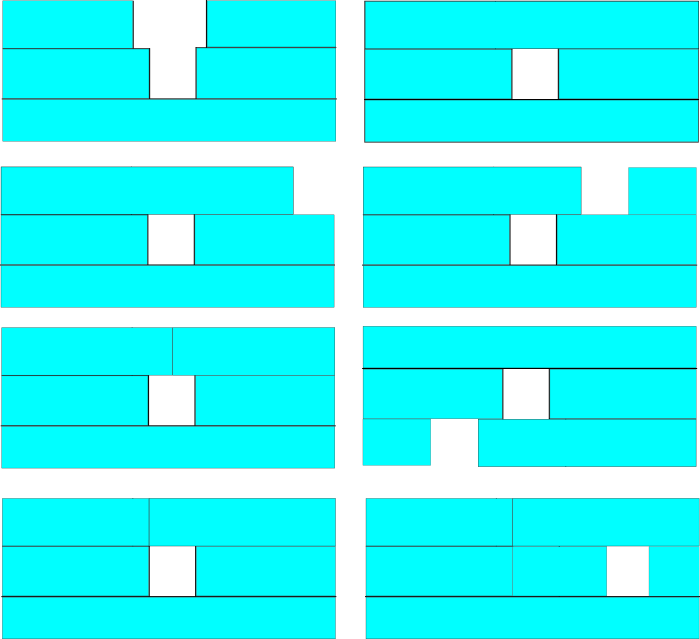
\includegraphics[width=0.7\textwidth]{mur.png}
	\caption{A number of invalid (left) and valid (right) walls.}
  \label{fig:sample}
\end{figure}

Given a proposal for how the wall should look, determine whether the wall is a valid wall.

\section*{Input}
The first line contains two integers $W$ and $H$ --- the width and height of the wall.

The following $H$ lines describe the rows of the wall.
Each line starts with an integer $B \ge 1$, the number of blocks on the row.
This is followed by $B$ pairs of integers $P_j, L_j$, the (zero-indexed) position and length of the $j$th block on the row. These will be given in increasing $P_j$ order, i.e.\ from left to right.
No blocks will overlap or extend outside the wall.

The rows are given from the bottom up --- i.e.\ the first row in the input is the bottom row of the wall.

Let the sum of the number of blocks over all rows be $N$.
This value has limits in the scoring table.

\section*{Output}
You shall output \texttt{YES} if the wall is valid, and \texttt{NO} if it is not.

\section*{Scoring}
Your solution will be tested on a set of test groups. To earn points for a group, you must pass all test cases in that group.

\noindent
\begin{tabular}{| l | l | l | l |}
\hline
Group & Points & Constraints & Other \\ \hline
1     & 31         & $1 \le N, W, H \le 100\,000$ & No gap occurs directly above another gap \\ \hline
2     & 34         & $1 \le N, W, H \le 1\,000$ & \\ \hline
3     & 35         & $1 \le N, W, H \le 100\,000$ & \\ \hline
\end{tabular}

\section*{Explanation of Samples}
The first four samples correspond to the four invalid walls on the left in the image.
The last four samples correspond to the four valid walls on the right in the image.
